\documentclass[12pt,fleqn]{article}\usepackage{../../common}
\begin{document}
Katı-Gövde Simülasyonu

Bir örnek gövde üzerinde simülasyon yapmaya uğraşalım. Elimizde bir simit, ya da
geometride torus denen bir şekil var. Bu dosya STL denen bir format içinde,
detaylar için [1]. Torus STL şekli içiçe geçmiş üçgenler ile tanımlı, bu
üçgenlerin herbirine dik olan normal vektörü biliyoruz. O üçgenlerden birinin
orta noktasından çıkan vektörlerden birini ters çevirirsek, o noktaya o yönde
bir kuvvet uyguladığımızı hayal edelim, ve simülasyonun geri kalanını bu
noktadan devam ettirelim.

\begin{minted}[fontsize=\footnotesize]{python}
from stl import mesh

your_mesh = mesh.Mesh.from_file('torus.stl')

prop = your_mesh.get_mass_properties()
print ('hacim',np.round(prop[0],3))
print ('\nyercekim merkezi (COG)',np.round(prop[1],3))
print ('\nCOG noktasinda atalet matrisi')
print (np.round(prop[2],3))
\end{minted}

\begin{verbatim}
hacim 4.918

yercekim merkezi (COG) [-0.  0. -0.]

COG noktasinda atalet matrisi
[[ 3.223 -0.     0.   ]
 [-0.     3.223  0.   ]
 [ 0.     0.     5.832]]
\end{verbatim}

COG'nin sıfır noktasında olması mantıklı çünkü STL dosyasında simit şekli oraya
konmuş, ve simit şekli simetrik bir şekil.

\begin{minted}[fontsize=\footnotesize]{python}
import matplotlib.pyplot as plt
from mpl_toolkits import mplot3d

fig = plt.figure()
axes = mplot3d.Axes3D(fig)

scale = your_mesh.points.flatten()
axes.add_collection3d(mplot3d.art3d.Poly3DCollection(your_mesh.vectors,alpha=0.3))
axes.auto_scale_xyz(scale, scale, scale)

def plot_vector(fig, orig, v, color='blue'):
   ax = fig.gca(projection='3d')
   orig = np.array(orig); v=np.array(v)
   ax.quiver(orig[0], orig[1], orig[2], v[0], v[1], v[2],color=color)
   ax = fig.gca(projection='3d')  
   return fig

LIM = 5
axes.set_xlim(-LIM,LIM);axes.set_ylim(-LIM,LIM);axes.set_zlim(-LIM,LIM)

SCALE = 4
tidx = 2000
o = np.mean(your_mesh.vectors[tidx],axis=0)
axes.plot (o[0],o[1],o[2],'gd')
n = your_mesh.get_unit_normals()[tidx]
plot_vector(fig, o, n*SCALE)
plot_vector(fig, o, -n*SCALE, color='red')
axes.view_init(azim=84,elev=28)

plt.savefig('phy_005_basics_04_05.png')
\end{minted}

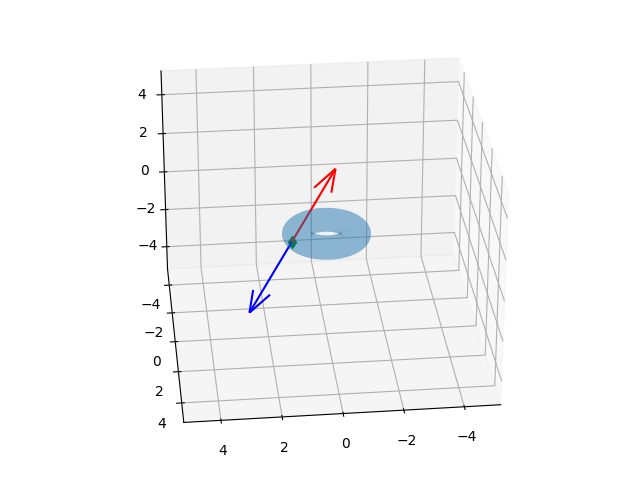
\includegraphics[width=20em]{phy_005_basics_04_05.png}

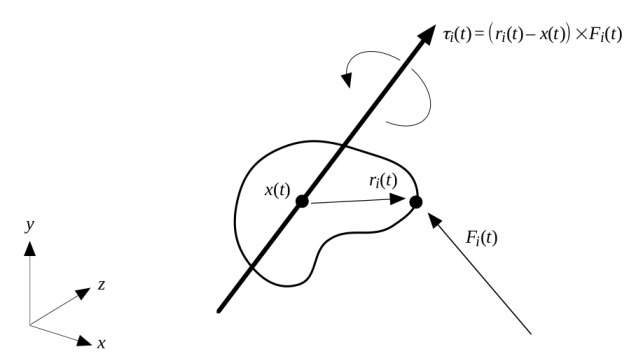
\includegraphics[width=25em]{phy_008_sim_rigbod_01.png}

\begin{minted}[fontsize=\footnotesize]{python}
import numpy.linalg as lin
from scipy.integrate import odeint

def skew(a):
   return np.array([[0,-a[2],a[1]],[a[2],0,-a[0]],[-a[1],a[0],0]])

prop = your_mesh.get_mass_properties()
R0 = np.eye(3,3)
omega = np.array([1,1,1])
skew_omega = skew(omega)
   
def rhs(u,t):   
   R1x,R1y,R1z,R2x,R2y,R2z,R3x,R3y,R3z = u
   R = np.array([R1x,R1y,R1z,R2x,R2y,R2z,R3x,R3y,R3z])
   R = R.reshape((3,3)).T
   res = np.dot(skew_omega, R)
   return list(res.T.flatten())

t=np.linspace(0.0, 1.0, 3)
R0 = np.eye(3,3)
u0 = R0.flatten()
u1=odeint(rhs,list(u0),t)
print (u1)
\end{minted}

\begin{verbatim}
[[ 1.          0.          0.          0.          1.          0.
   0.          0.          1.        ]
 [ 0.76523954  0.55718255 -0.32242209 -0.32242209  0.76523954  0.55718255
   0.55718255 -0.32242209  0.76523954]
 [ 0.22629566  0.95671225 -0.18300792 -0.18300792  0.22629566  0.95671225
   0.95671225 -0.18300792  0.22629566]]
\end{verbatim}















[devam edecek]

Kaynaklar

[1] Bayramlı, {\em 3D Baskıya Hazır CAD Tasarımlarına Erişmek, Numpy-STL},
    \url{https://burakbayramli.github.io/dersblog/sk/2020/08/numpy-stl.html}

[2] Witkin, {\em Physically Based Modeling}

\end{document}



